\section{\acs{NMR} Data Processing and Analysis}
\begin{remark}
    In contexts where \ac{1D} datasets are considered specifically, the
    redundant dimension index $^{(1)}$ will be neglected for conciseness.
\end{remark}
\subsection{Processing NMR Data}
\label{subsec:nmr-proc}
The typical means of processing \ac{NMR} data is to
transform the time (measured) domain \ac{FID} into the frequency
domain, yielding an \emph{\ac{NMR} spectrum}. This is achieved through
application of the \ac{FT}. The \ac{FT} converts a continuous function over
time $t$, to one over frequency $F$ as follows\footnote{
    In general, the \ac{FT} is defined over the range $(-\infty, \infty)$.
    Since \ac{NMR} data isn't defined for $t < 0$, the \ac{FT} has been defined
    over the range  $[0, \infty)$ instead.
}:
\begin{equation}
    s(F) =  \int_{0}^{\infty} x(t) \exp(
        -2 \pi \iu t F
        ) \mathrm{d} t
\end{equation}
In practice, the discrete signal acquired by the spectrometer is processed
using the \ac{DFT}:
\begin{equation}
    s_n = \sum_{k=0}^{N-1} x_k \exp \left(
            -\frac{2 \pi \iu k n}{N} \right)
            \quad \forall n \in \lbrace 0, \cdots, N-1 \rbrace.
\end{equation}
The \ac{FT} of a continuous exponentially-damped complex sinusoid
takes the form of a \emph{Lorentzian}:
\begin{subequations}
    \begin{gather}
        s(F) = \int_0^{\infty}
            a \exp(\iu \phi) \exp((2 \pi \iu f - \eta)t)
            \exp(-2 \pi \iu t F)
            \mathrm{d} t,\\
        s(F) = \frac{a \exp(\iu \phi) }
            {\eta + 2 \pi \iu (f - F)}.
    \end{gather}
    \label{eq:lorentzian}%
\end{subequations}
When processing discrete data, the \ac{DFT} of an \ac{FID}
features a vertical offset, such that the baseline does not sit at
0. This results from only possessing data for positive
values of $t$, rather than having a ``full echo'', where negative values of
$t$ are accounted for too. Fortunately, this can be corrected easily by
halving the initial point of the \ac{FID} prior to \ac{DFT}\cite{Tang1994}.
The \ac{FT} is a linear function, such that the
\ac{FT} of a summation of signals is equivalent to the summation of all
the individual \ac{FT}s of the signals. A corollary is that an \ac{NMR}
spectrum comprises a series of Lorentzian ``peaks'', located at the frequencies
of the signals in the \ac{FID}:
\begin{equation}
    s\left(F\right) = \sum_{m=1}^{M}
    \frac{\amexpphim}
    {\eta_m + 2 \pi \iu (f_m - F)}.
    \label{eq:ft-summation}%
\end{equation}
The \ac{FT} is a very attractive means of processing \ac{NMR} data, as it
presents the data in a format which is human-interpretable; the basic
rules describing how chemical structure is mapped to \ac{NMR} spectra
is a fundamental skill that experimentalists in many fields
require\cite{Hore2015b}.
Due to innate properties of the \ac{NMR} experiment,
as well as issues arising from analysing discrete data, the \ac{FT} of
the raw \ac{FID} has undesirable
characteristics without further manipulation. Additional processing
steps that are frequently applied to \ac{NMR} data are now outlined, in the
usual order that they are employed. Apodisation and zero filling
are applied prior to \ac{FT} (i.e. to the \ac{FID}), while phase
correction and baseline correction are applied to the resultant spectrum.

\subsubsection{Apodisation}
Apodisation refers to the process of mutating a signal by multiplying it with a
specified function, often called a \emph{window function}\cite[Section
3.2.7]{Claridge2016}, as a means of enhancing either the sensitivity or the
resolution of the final spectrum, albeit at the cost of worsening the other
feature.

\paragraph{Sensitivity Enhancement} As \iac{FID} progresses with time, the
contributions from the desirable signal ($\bx$) and experimental noise ($\bw$)
becomes more weighted towards the noise, as spin relaxation phenomena attenuate
the signal.  Multiplying the \ac{FID} with a function which decreases in value
with time can be used to enhance the \ac{SNR} of the \ac{FID}, as later points
which are heavily noise-weighted are suppressed. The most common function to
achieve this is the negative exponential, in which a given point is multiplied
by $\exp(-\nicefrac{k n}{N - 1})$.  $k$ is referred to as the line broadening
factor, since the increased damping applied to the \ac{FID} causes the
linewidth of the spectral peaks to increase (see
\cref{fig:amp-phase-freq-damp}.d).

\paragraph{Resolution Enhancement} By contrast, resolution enhancement can be
achieved by applying a window function that artificially reduces the rate of
signal decay. It is possible to do this by attenuating the early datapoints in
\ac{FID}. Popular examples of window functions for resolution enhancement are
the Lorentz-Gauss function, which bestows a sharper, Gaussian shape to the
peaks, and the sine-bell, which is commonly used in multidimensional
experiments.  Since the initial points in the \ac{FID} are reduced in
magnitude, these window functions decrease the sensitivity of the resulting
spectra.

By being defined to decay to a sufficiently small value (or $0$ itself) at the
end of
the \ac{FID}, window functions are also able to suppress \emph{truncation
artefacts}, which appear when the \ac{FID} still possesses appreciable signal
amplitude at the end of the acquisition period. Truncated \acp{FID} produce
spectra with peaks of a form that is akin to the convolution of the \ac{FT} of
the untruncated \ac{FID}, with the \ac{FT} of a box-function, which has the
form of a sinc function ($\nicefrac{\sin(x)}{x}$). The resulting artefacts
are often referred to as \emph{sinc wiggles} for this reason.

\subsubsection{Zero-filling}
Zero-filling refers to the process of appending zeros to the end of an
\ac{FID}. One reason why this is often done is to ensure that the number of
points in the \ac{FID} is a power of 2, making the \ac{FID} of an optimal size
for processing by divide and conquer methods like the Cooley-Tukey
algorithm\cite{Cooley1965}. Beyond this, it is actually
possible to enhance the information content of the real component of the
spectrum if an \ac{FID} comprising $2^{x-1} < N \leq 2^x$ points is zero-filled
to $2^{x+1}$ points\cite{Bartholdi1973}. By doing this, the real and imaginary
components of
the spectrum become causally linked; the real component can be derived from the
imaginary component and vice versa via the Hilbert Transform, in accordance
with the Kramers-Kronig relations.
Zero-filling beyond a factor of 2 can bestow a
cosmetic improvement to spectra, but it does not incorporate any new
information into them; any additional points are simply interpolations.

\subsubsection{Phase correction}
The real and imaginary components of \cref{eq:ft-summation} are as follows:
\begin{subequations}
    \begin{gather}
        \Re(s(F)) = \sum_m
        a_m (\cos(\phi_m) \mathcal{A}_m(F) + \sin(\phi_m) \mathcal{D}_m(F)),\\
        \Im(s(F)) = \sum_m
        a_m (\sin(\phi_m) \mathcal{A}_m(F) - \cos(\phi_m) \mathcal{D}_m(F)),
    \end{gather}
\end{subequations}
where $\mathcal{A}_m$ and  $\mathcal{D}_m$ denote \emph{absorption} and
\emph{dispersion} Lorentzians, respectively:
\begin{subequations}
    \begin{gather}
        \mathcal{A}_m(F) = \frac{\eta_m}{\eta_m^2 + 4 \pi^2 (f_m - F)^2},\\
        \mathcal{D}_m(F) = \frac{2 \pi (f_m - F)}{\eta_m^2 + 4 \pi^2 (f_m - F)^2}.
    \end{gather}
\end{subequations}
As illustrated most clearly in \cref{fig:amp-phase-freq-damp}.c2, a peak with
an absorption lineshape is far more desirable than one with a dispersion
lineshape for two key reasons:
\begin{enumerate}
    \item Its maximum corresponds to the signal frequency, while a dispersion
        Lorentzian has a magnitude of $0$ at this frequency.
    \item It decays more rapidly and therefore exhibits better resolution;
        at large frequency offsets (i.e. when $\lvert F - f_m \rvert$ is
        notably greater than \qty{0}{\hertz}) absorption Lorentzians decay at
        a rate $\propto \nicefrac{1}{(f_m - F)}^2$, while dispersive
        Lorentzians decay at a rate $\propto \nicefrac{1}{\lvert f_m - F \rvert}$.
\end{enumerate}
Generating a spectrum whose real component comprises peaks which all possess
absorption Lorentzians is therefore desired, which is possible if all signals
have a phase of \ang{0}:
\begin{subequations}
    \begin{gather}
        \Re(s(F)) = \sum_m a_m \mathcal{A}_m(F),\label{eq:absorption}\\
        \Im(s(F)) = -\sum_m a_m \mathcal{D}_m(F).\label{eq:dispersion}
    \end{gather}
\end{subequations}
For the majority of \ac{NMR} experiments\footnote{
     An example of an exception to this rule is when \acl{FS} pulses are applied,
     which generate datasets with quadratic phase behaviour. This is discussed
     in more detail in \cref{sec:bbqchili}.
}, the contributing signals possess phases which depend linearly on their
frequencies, i.e.
\begin{equation}
    \phi_m = \Phi_0 + \Phi_1 f_m,
\end{equation}
where $\Phi_0 \in (-\pi, \pi]$ and $\Phi_1 \in \mathbb{R}$ are zero- and
first-order phase terms.
Phase correction refers to the process in which $\Phi_0$ and $\Phi_1$ are
determined by inspecting the appearance of the spectrum
$\symbf{s}_{\phi}$ for different values of $p_0$ and  $p_1$, according to
\begin{equation}
    s_{\phi,n} = s_n
    \exp\left(-\iu \left(p_0 + \frac{p_1 n}{N - 1}\right)\right).
\end{equation}
When $p_0 = \Phi_0$ and  $p_1 = \Phi_1$, the spectrum will be correctly phased.

\subsubsection{Baseline correction}
The baseline of an \ac{NMR} spectrum is used to describe regions where
no discernible peaks reside (i.e. only experimental noise exists).
Baseline distortion refers to scenarios in which the baseline, rather
than exhibiting a flat profile with an average of zero, has some other form.
There a number of potential causes of baseline distortion, including
``clipping'' of the initial points due to excessive receiver gain,
and pulse breakthrough.
Whatever the cause(s), it is typically a corruption of the initial points in
the \ac{FID} that causes baseline distortion.
It is common to apply a baseline correction algorithm to negate any distortion,
which involves adding a spline or high-order polynomial to the spectrum.
One class of approaches which are used widely involve the two principal steps
of (a) determining spectral regions which are part of the baseline, and (b)
fitting the baseline regions to the chosen
function before subtracting the fit from the
spectrum\cite{Dietrich1991,Cobas2006}.

\subsection{Processing Multidimensional Data}
\label{subsec:multidim}
As for \ac{1D} datasets, it is desirable that multidimensional \ac{NMR} spectra
feature peaks which are frequency discriminated, and comprise pure
absorption lineshapes in each dimension.
A description of how this can be achieved for both amplitude- and
phase-modulated datasets is now given, through the consideration of \ac{2D}
\acp{FID} which comprise a single signal.

\subsubsection{Amplitude-Modulated Datasets}
It is clear that a cosine-modulated signal, given by \cref{eq:general-fid}
with $D=2$ and $\zeta^{(1)} = \cos(\cdot)$ cannot achieve frequency
discrimination in the indirect dimension, on account of the relation
\begin{equation}
    \cos\left(2 \pi \fone \tone\right) =
    \frac{\exp\left(2 \pi \iu \fone \tone \right) + \exp\left(-2 \pi \iu \fone \tone \right)}{2}
\end{equation}
Performing \ac{FT} on such a signal in both dimensions leads to a spectrum
whose real component comprises two peaks: one at the true resonance frequency
$\left(\fone, \ftwo\right)$, and the other at the mirror-image frequency in the
indirect dimension, $(2\foffone - \fone, \ftwo)$. On top of this, the
peaks possess a mixture of absorption and dispersion character, with the
resultant peak shape often referred to as \emph{phase twist}\cite{Keeler1985}.
A spectrum of this form is presented in \cref{fig:2d-lineshapes}.a.
It is possible to generate pure absorption peaks by applying \ac{FT} in the
direct dimension, setting the imaginary component to zero, and finally
applying \ac{FT} in the indirect dimension. The real component of the result
(\cref{fig:2d-lineshapes}.b) is referred to as a double absorption spectrum.

For frequency discrimination, it is necessary to also possess the
analogous sine-modulated signal ($\zeta^{(1)} = \sin(\cdot)$) as this
achieves the necessary quadrature detection in the indirect dimension. For
numerous multidimensional experiments, repeating the
pulse sequence with methodical adjustments to the phases of particular pulses
in a process referred to as \emph{phase cycling} enables
this\cite[Chapter 11]{Keeler2010}.
Applying the same processing as that which achieved the double absorption
spectrum for the cosine-modulated case generates a spectrum whose imaginary
component features two peaks, but with opposite signs
(\cref{fig:2d-lineshapes}.c) on account of sine being an odd function.
It then becomes possible to generate a frequency discriminated spectrum by
subtracting the sine spectrum from the cosine spectrum
(\cref{fig:2d-lineshapes}.d).

\begin{figure}
    \centering
    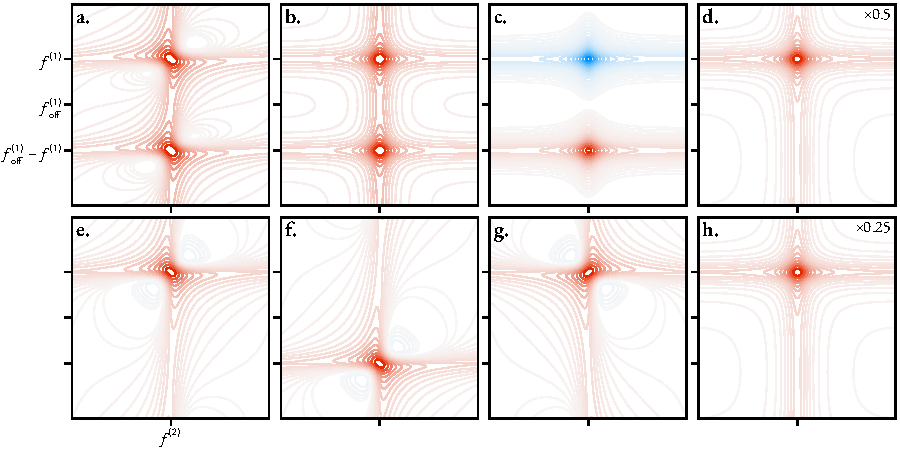
\includegraphics{2d_lineshapes/2d_lineshapes.pdf}
    \caption[
        Spectra acquired from amplitude- and phase-modulated \acs{2D} signals
        which have been processed in different ways.
    ]{
        Spectra acquired from amplitude- and phase- modulated \acs{2D} signals.
        Red contour lines denote positive values, while blue contours denote
        negative values.
        \textbf{a.} The \ac{FT} of a cosine-modulated \ac{FID}, featuring peaks
        both at the true resonance frequency ($\fone$) and the mirrored
        frequency ($2\foffone - \fone_{\vphantom{off}}$), and with phase-twist lineshapes.
        \textbf{b.} Double-absorption spectrum generated by applying \ac{FT}
        in the direct dimension, setting the imaginary component to zero,
        applying \ac{FT} in the indirect dimension, and retaining the real
        component.
        \textbf{c.} Spectrum acquired with the same processing method as in
        \textbf{b.} but with a sine-modulated \ac{FID}, and with the imaginary
        component retained.
        \textbf{d.} The subtraction of the spectrum in \textbf{c.} from that in
        \textbf{b.} leads to a spectrum with frequency discrimination and a
        pure absorption lineshape.
        \textbf{e.} The \ac{FT} of a positive phase-modulated \ac{FID},
        exhibiting frequency discrimination, but with a phase twist shape.
        \textbf{f.} The \ac{FT} of a negative phase-modulated \ac{FID}.
        \textbf{g.} The spectrum in \textbf{f.} inverted along the indirect
        axis, about $\foffone$.
        \textbf{h.} The summation of \textbf{e.} and \textbf{g.} generates a
        spectrum with an absorption lineshape.
    }
    \label{fig:2d-lineshapes}
\end{figure}

\subsubsection{Phase-modulated signals}

A positive (\emph{hypercomplex}) phase-modulated signal ($\zeta^{(1)}
= \exp(\iu \cdot)$) is frequency discriminated due to
its quadrature nature in the indirect dimension. However, a direct \ac{FT} of
such a signal in both dimensions leads to a peak with a phase twist lineshape,
with no means of
separating the absorption and dispersion contributions (\cref{fig:2d-lineshapes}.e). Certain pulse
sequences, including \ac{2DJ} spectroscopy\cite{Aue1976,Morris2009} (see
\cref{chap:cupid}) and
\ac{COSY}\cite{Jeener1971,Jeener2016,Aue1976a} produce hypercomplex datasets,
and the conventional means of processing is simply to display the
spectrum in \emph{magnitude-mode}, where the absolute value of each complex
point is plotted. While the phase twist shapes are removed by doing this, the
resulting peaks have broad ``wings'', due to the influence of the
dispersive components, and they also suffer from significant non-linearities.
In scenarios where it is possible, it is desirable to acquire the equivalent
negative signal ($\zeta^{(1)} = \exp(-\iu \cdot)$), whose \ac{FT} leads to a
peak with the same phase twist form, but centered at $2\foffone - \fone$
(\cref{fig:2d-lineshapes}.f).
Inverting this spectrum about $\foffone$ (\cref{fig:2d-lineshapes}.g), and summing with the positive
spectrum nullifies the dispersive contribution, generating a spectrum with an
absorption lineshape\cite{Davis1992} (\cref{fig:2d-lineshapes}.h).

The concepts described here for \ac{2D} signals can be extended for the
processing of \ac{NMR} datasets with any number of dimensions, provided that in
each indirect dimension, the requisite pair of amplitude- or phase-modulated
signals exist. As such, a set of $2^{D-1}$ signals need to be acquired to
produce $D$-dimensional spectra with absorption-mode peaks in all dimensions.

\subsection{Analysing NMR Data}
\label{subsec:estimation-techniques}
The amount of detail required from an \ac{NMR} dataset depends on
the user's requirements. In synthetic organic chemistry, \ac{NMR} is often used
simply as a means of verifying that a particular step in a synthetic pathway
was successful. A simple inspection of peak locations and splittings due to
scalar couplings in the spectrum may be sufficient to verify that the desired
molecule was created. However, in many situations a detailed quantitative
description of the data is desired. Some examples include:
\begin{itemize}
    \item Deducing the relative concentrations of molecules in a mixture,
        with application in areas such as reaction
        monitoring\cite{Bernstein2016} and metabolomics\cite{Emwas2019}.
        In these circumstances, it is necessary to deduce the relative
        amplitudes of the signals in the data.
    \item Determining properties such as translational diffusion coefficients
        and relaxation rates, which can be achieved using a suite of \ac{2D}
        experiments in which each successive \ac{1D} \acp{FID} exhibit
        attenuations in their signal amplitudes (these are discussed in
        \cref{sec:seq}).  Typical approaches to analysing these datasets
        requires identification of the frequencies of spectral peaks of
        interest, from which amplitudes are extracted and fit to a
        function which models the expected decay profile of the data.
\end{itemize}

Most \ac{NMR} users are principally interested in the integrals and positions
of peaks in spectra\footnote{
    There may be some situations where the linewidth of the peaks are of
    interest too. An absorption Lorentzian produced from an
    exponentially-damped complex sinusoid with a damping factor $\eta$ will
    have a linewidth at half its maximum intensity of $\nicefrac{\eta}{\pi}$.
    Peak linewidths give an insight into the rate of transverse
    relaxation ($T_2$) associated with a given spin.
}.
Integrals are usually computed by applying a discrete integration method such
as Simpson's rule on a collection of consecutive points in the spectrum which
lie within user-specified regions.
The most rudimentary form of ``peak picking''\,---\,beyond the user
simply defining where peaks are by inspecting the spectrum\,---\,involves
assessing where relative maxima exist in the spectrum, subject to
tolerances which aim to prevent blips due to noise being categorised as
peaks.

While integration and peak picking works adequately for high \ac{SNR} spectra
featuring very well-separated peaks, in most practical situations accurate
quantification of individual signals is impossible using this approach,
principally due to the inherently poor resolution associated with the
\ac{FT}.
For this reason, considerable interest has been given to the development of
techniques which are better-able to quantify \ac{NMR} datasets, by attempting
to estimate the optimal set of parameters $\bth$ which describe them\footnote{
    The process of estimating the parameters describing an \ac{NMR}
    dataset is often referred to as \emph{deconvolution}. The term is not used
    here as it is a misnomer; deconvolution is simply the inverse operation of
    convolution, and has nothing to do with estimating the parameters which
    describe a dataset. Equivalently, \emph{convolution} is not the process of
    generating an \ac{NMR} dataset by summing a number of complex
    sinusoids, though it is often described as so in the literature.
}.
Here, a summary of some of the most prominent methods for quantifying \ac{NMR}
data are given. Attention is primarily given to methods which consider
time-domain data; for reasons that will be explained shortly, time-domain
estimation is the focus of this work.

\subsubsection{Linear Prediction}
\Ac{LP}\cite{Stephenson1988,Koehl1999,Marion1989b,Zhu1992} is a procedure which
is widely used in \ac{NMR} data analysis for the purposes of (a) propagating
\iac{FID} further in time in order to reduce the presence of truncation
artefacts without the reliance on severe apodisation, and/or (b) correcting the
commonly corrupted initial points of the \ac{FID}, as a means of improving the
spectral baseline. \ac{LP} is notably different to the other methods presented
here; while the other approaches aim to determine the parameters defining each
contributing signal in the \ac{FID}, \ac{LP} is used to provide a holistic
picture, describing how a datapoint in the \ac{FID} is related to those
which precede or succeed it.

\ac{LP} stems from the concept that \iac{FID} can be described as
an \ac{AR} process, meaning that a given sample from the dataset is a linear
combination of an appropriate number $L$ of previous samples. For a \ac{1D}
\ac{FID}, it is assumed that
\begin{equation}
    y_n = \sum_{l=1}^{L}
    c_l y_{n-l} + e_l \quad
    \forall n \in \lbrace L, L + 1, \cdots, N - 1 \rbrace,
    \label{eq:forward-lp}
\end{equation}
where $L \in
\mathbb{N}$ defines the order of the linear estimator, and $\symbf{c} \in
\mathbb{R}^{L}$ is a set of \emph{forward} \ac{LP} coefficients. $\symbf{e} \in
\mathbb{R}^L$ is a set of parameters, often called the innovations,
which account of error in the \ac{LP} model. A datapoint can also be described
by a linear combination of subsequent points, using the set of \emph{backward}
\ac{LP} coefficients $\symbf{b} \in \mathbb{R}^L$:
\begin{equation}
    y_n = \sum_{l=1}^{L}
    b_l y_{n+l} + e_l \quad
    \forall n \in \lbrace 0, 1, \cdots, N - L - 1 \rbrace.
    \label{eq:backward-lp}
\end{equation}
Determining
the \ac{LP} coefficients enables the estimation of \ac{FID} values beyond the
data actually acquired ($n > N - 1$), as well as to replace
datapoints which are anticipated to be corrupted. It should be noted that
\cref{eq:forward-lp,eq:backward-lp} are only technically valid for
\acp{FID} without any corruption from experimental noise. Noisy datasets are
instead an example of an \ac{ARMA} process. Despite this, due to the greater
simplicity of the \ac{AR} model, it is far more common to employ this, with
effective results attainable as long as the data is not extrapolated by too
great an extent. The most common means of performing \ac{LP} is by solving the
Yule-Walker equations\cite{Yule1927,Walker1931}, which describe the
relationship between the signal autocorrelation coefficients and the \ac{LP}
coefficients\cite[Section 3.3]{Koehl1999}, with the Levinson-Durbin algorithm
providing an efficient means of solving the
equations\cite{Levinson1946,Durbin1960}.

\subsubsection{\acs{SVD}-based methods}
\acused{SVD}
Some of the most prevalent methods for \ac{NMR} estimation involve
\ul{\emph{singular value decomposition} (SVD)}
as a key component. For each of these methods,
\ac{SVD} is applied to a \ul{Hankel} or \ul{Toeplitz matrix} containing the \ac{FID}.
Above a certain \ac{SNR} threshold, it is found that the singular values in the
data matrix corresponding to signal are larger than those related to noise, and
as such forming a low-\ul{rank} approximation of the data matrix nullifies
contributions from noise in the parameter estimate. The degree of truncation
required is dependent on the suspected \emph{model order} (i.e. the number of
contributing signals, $M$) of the dataset, which must
be supplied, or determined by some appropriate metric. All the \ac{SVD}-based
techniques determine the non-linear parameters (frequencies and
damping factors, incorporated in the signal poles) associated with the dataset.
Subsequently, the amplitudes and phases can be computed by solving a linear
least-squares problem involving a \ul{Vandermonde matrix} of the signal poles:
\begin{subequations}
    \begin{gather}
        \symbf{\alpha} = \symbf{Z}^+ \symbf{y},\\
        \symbf{Z} = \begin{bmatrix}
            1 & 1 & \cdots & 1 \\
            z_1^1 & z_2^1 & \cdots & z_M^1\\
            \vdots & \vdots & \ddots & \vdots\\
            z_1^{N-1} & z_2^{N-1} & \cdots & z_M^{N-1}\\
            \end{bmatrix}.
    \end{gather}
    \label{eq:complex-amplitudes}
\end{subequations}

Both \ac{LPSVD}\cite{Kumaresan1982,Kumaresan1983} and
\ac{HSVD}\cite{Kung1983} have be used extensively in the field of \ac{MRS}
after introduction by Barkhuijsen and
co-workers\cite{Barkhuijsen1985a,Barkhuijsen1985b,Barkhuijsen1987,Beer1988,Pijnappel1992}.
With
\ac{LPSVD}, the signal poles are determined by finding the roots of a
polynomial which features the backward \ac{LP} coefficients associated with the
signal, in a similar fashion to the classic Prony method\cite{Prony1795}.
\ac{HSVD} is based on the ``state-space'' principle, which generated interest
in part because it meant that the computationally costly polynomial rooting
step in \ac{LPSVD} was avoided.
A further technique in this category, the
\ac{MPM}\cite{Hua1990,Hua1990b,Hua1991} is based on solving a generalised
eigenvalue problem.  Pines and co-workers introduced the \ac{ITMPM}\cite{Lin1997},
for use in \ac{NMR}, which combines the \ac{MPM} with a method for estimating
the model order, such that no \textit{a priori} information is required from
the user.  Recently, the \ac{MPM} has been employed for the analysis of
\ac{NMR} relaxometry data\cite{Fricke2020, Wortge2023}.  Outlines of the
\ac{MPM} and its \ac{2D} equivalent, the \ac{MMEMPM}\cite{Hua1992,Chen2007} are
provided in detail in \cref{subsec:mpm}.

% separating contributions from deterministic
% signal in the \ac{FID} from experimental noise.

% \paragraph{\acs{LPSVD}} \Ac{LPSVD} was proposed by Kumaresan
% and Tufts\cite{Kumaresan1982}, and introduced to \ac{NMR} by Barkhuijsen and
% co-workers\cite{Barkhuijsen1985a,Barkhuijsen1985b}. Given the backward \ac{LP}
% assumption above, consider the set of linear equations for a \emph{noiseless}
% \ac{FID} $\symbf{x} \in \mathbb{C}^{N}$:
% \begin{equation}
%   \label{eq:lineqs}
%   \underbrace{
%       \begin{bmatrix}
%         x_1^* & x_2^* & \cdots & x_L^*\\
%         x_2^* & x_3^* & \cdots & x_{L+1}^*\\
%         \vdots & \vdots & \ddots & \vdots\\
%         x_{N-L}^* & x_{N-L+1}^* & \cdots & x_{N-1}^*\\
%       \end{bmatrix}
%   }_{\symbf{A}}
%   \underbrace{
%       \begin{bmatrix}
%         b_1\\
%         b_2\\
%         \vdots\\
%         b_L
%       \end{bmatrix}
%   }_{\symbf{b}}
%   = -
%   \underbrace{
%       \begin{bmatrix}
%         x_0^*\\
%         x_1^*\\
%         \vdots\\
%         x_{N-L-1}^*
%       \end{bmatrix}
%   }_{\symbf{h}},
% \end{equation}
% with $L \geq M$.
% This equation can be augmented into the form $\symbf{A}^{\prime}
% \symbf{b}^{\prime} = \symbf{0}$, with $\symbf{A}^{\prime} = \left[ \symbf{h}
% \vert \symbf{A} \right]$ and $\symbf{b}^{\prime} = \left[1 \hspace*{4pt}
% \symbf{b}^{\mathrm{T}}\right]^{\mathrm{T}}$.
% Any row of $\symbf{A}^{\prime}$ can be written as the linear
% combination of $M$ linearly independent vectors $\symbf{r}_m\ \forall m \in
% \{1, \cdots, M\}$\cite{Kumaresan1983}:
% \begin{equation}
%   \symbf{r}_m =
%   \begin{bmatrix}
%       1 & z_m^* & (z_m^2)^* & \cdots & (z_m^L)^*
%   \end{bmatrix},
% \end{equation}
% where $z_m$ is the signal pole of the $m$\textsuperscript{th} signal, given by
% \cref{eq:signal-pole}.
% This means that the rank of $\symbf{A}^{\prime}$ is $M$, provided it possesses
% at least $M$ rows ($M \leq N - L$). Because $\symbf{b}^{\prime}$ lies in the
% null space of $\symbf{A}^{\prime}$, $\symbf{r}_m
% \symbf{b}^{\prime} = 0$, such that the following holds:
% \begin{equation}
%   \label{eq:lincom}
%   1 + b_1 z_m^* + b_2 (z_m^2)^* + \cdots + b_L (z_m^L)^* = 0
% \end{equation}
% Therefore, the signal poles can be determined by finding
% the roots of the polynomial $B(\zeta)$:
% \begin{equation}
%   B(\zeta) = 1 + b_1 \zeta^{-1} + b_2 \zeta^{-2} + \cdots + b_L \zeta^{-L}.
% \end{equation}
% The roots of $B(\zeta)$ will occur whenever $\zeta = \left(z_m^{-1}\right)^*\
% \forall m \in \{1, \cdots, M\}$.

% The prediction coefficient vector $\symbf{b}$ still needs to be determined.
% \cref{eq:lineqs} implies that $\symbf{b}$ can be determined by employing
% linear lest squares:
% \begin{equation}
%   \symbf{b} = - \mathbf{A}^+ \symbf{h}.
% \end{equation}
% However, in the case of real signals which are corrupted with noise $\symbf{y}
% \in \mathbb{C}^N$, noise
% would be incorporated into the solution of $\symbf{b}$. To mitigate this, a
% low-rank approximation of $\symbf{A}$ is produced, in an attempt to purge
% contributions from noise, and retain only contributions from the $M$ signals in
% the data. More information on the \ac{SVD} and its usefulness in generating
% low-rank approximations of matrices can found found in \cref{subsec:mpm} and
% \cref{subsec:linear-algebra}.
% The vector of prediction coefficients is determined by:
% \begin{equation}
%     \symbf{b} = - \sum_{m=1}^M \sigma_m^{-1 \vphantom{\dagger}} \left[
%     \symbf{u}_m^{\dagger} \symbf{h} \right] \symbf{v}_m^{\vphantom{\dagger}},
% \end{equation}
% where $\sigma_m$ is the  $m$\textsuperscript{th} most significant singular
% value of $\symbf{A}$, and $\symbf{u}_m$ and $\symbf{v}_m$ are the corresponding
% right and left singular vectors, respectively. As will be illustrated in
% \cref{subsec:mpm}, the complex amplitudes associated with the \ac{FID} can be
% determined by solving a linear set of equations involving a Vandermonde matrix
% of the signal poles:
% \begin{subequations}
%     \begin{gather}
%         \symbf{\alpha} = \symbf{Z}^+ \symbf{y},\\
%         \symbf{Z} = \begin{bmatrix}
%             1 & 1 & \cdots & 1 \\
%             z_1^1 & z_2^1 & \cdots & z_M^1\\
%             \vdots & \vdots & \ddots & \vdots\\
%             z_1^{N-1} & z_2^{N-1} & \cdots & z_M^{N-1}\\
%             \end{bmatrix}
%     \end{gather}.
% \end{subequations}

% \paragraph{\acl{MPM}}
% The \ac{MPM}, developed by Hua and Sarkar, largely finds preference over
% \ac{LPSVD} and \ac{HSVD} nowadays

\subsubsection{Iterative Methods}
For problems involving nonlinear function fitting, the most widespread approaches
are iterative techniques. The \ac{VARPRO} method\cite{Golub1973} is such an
example, which has been applied extensively in the field of \ac{MRS}, following
its introduction by van der Veen and
co-workers\cite{VanDerVeen1988,Decannierec1994}. \ac{VARPRO}
relies on determining the following quantity, an example of a \ac{RSS} problem:
\begin{equation}
    \symbf{\theta}^{(*)} = \argmin_{\symbf{\theta} \in \mathbb{R}^{4M}}
        \left \lVert \symbf{y} - \symbf{x}(\symbf{\theta}) \right \rVert^2 \equiv
        \argmin_{\symbf{\theta} \in \mathbb{R}^{4M}} \left \lVert \symbf{y} - \symbf{Z}\symbf{\alpha} \right \rVert^2,
\end{equation}
where $\bthstar$ is the optimal set of parameters which describe the data,
often referred to as the \ul{\emph{maximum likelihood estimate} (MLE)}.
\acused{MLE}
The linear parameters, residing in the vector of complex amplitudes, can be
expressed as $\symbf{Z}^+\symbf{y}$ (see \cref{eq:complex-amplitudes}). By doing
this, it becomes possible to recast the optimisation problem to only solve for
the nonlinear terms:
\begin{subequations}
    \begin{gather}
        \symbf{\rho}^{(*)} =
            \argmin_{\symbf{\rho} \in \mathbb{R}^{2M}}
            \lVert \symbf{y} - \symbf{Z}\symbf{Z}^+\symbf{y} \rVert^2,\\
        \symbf{\rho} =
        \begin{bmatrix}
            \bdf\T & \bdeta\T
        \end{bmatrix}\T.
    \end{gather}
\end{subequations}
The \ac{LM} algorithm\cite{Levenberg1944, Marquardt1963} is
typically employed to perform the optimisation routine, with amplitudes and
phases determined with linear least squares afterwards.

For such a routine to be effective, a large amount of \textit{a priori}
information needs to be provided, in the form of a set of estimated frequencies
and damping factors in the data; iterative methods like the \ac{LM} algorithm
only tend to perform successfully if they start with a set of parameters
sufficiently close to the \ac{MLE} in the parameter space.
Further specifications can be supplied to \ac{VARPRO}, reflecting the
spectroscopist's knowledge of the signal under inspection. For example, damping
factors corresponding to signals that form a particular multiplet can be
constrained to be equal\,---\,a feature which is common in the \ac{NMR} of
small molecules. \Ac{AMARES} is an improvement of \ac{VARPRO}, as it
facilitates the imposition of a wider range of linear constraints on the
parameter set\cite{Vanhamme1997}; it is now established as one of the most
prominent means of quantifying \ac{MRS} signals.

There is not much precedent of using iterative methods in \ac{NMR} analysis,
despite its widespread adoption in \ac{MRS}. The main cause of this is probably due to
the requirement to supply a large amount of prior knowledge; in \ac{MRS}, it
is likely that the practitioner has an intimate understanding of the expected signals
which will be present in an acquired dataset, since all signals will derive
from species which make up the human metabolome, whose chemical shifts and multiplet
structures will be well-established. As \ch{^{31}P} is the most
common nucleus studied in \ac{MRS}, the number of potential species
contributing to datasets is reduced even further. Over many experiments, little
adjustment to the information provided to the optimiser will need to be given,
making the process facile. In \ac{NMR} experiments, there is a far greater
variation in the appearance of the data, such that the process of defining
\textit{a priori} information for each dataset of interest is likely to become
time-consuming and cumbersome. Furthermore, there is also a good possibility
that the expected form that the dataset adopts in unknown in \ac{NMR}, making
any method which requires intimate knowledge about the data worthless.

\subsubsection{Bayesian Methods}
\Ac{CRAFT}\cite{Krishnamurthy2013,Krishnamurthy2021} is a routine developed by
Krishnamurthy, inspired by previous work by
Bretthorst\cite{Bretthorst1990a,Bretthorst1990b,Bretthorst1990c,Bretthorst1991,Bretthorst1992},
for the parametric estimation of \acp{FID} based on the principle of Bayesian
inference.
In brief, \ac{CRAFT} consists of defining prior distributions for the signal
parameters, and gradually increasing the number of signal components in the
model until a maximisation of the posterior probably is achieved; through this
approach, both model order selection and parameter estimation are achieved
in tandem. In order to reduce the considerable computational burden associated
with the method, the complete \ac{FID} is downsampled into a series of
``sub-\acp{FID}'', with each sub-\ac{FID} being analysed separately.
\ac{CRAFT} has been extended for the consideration of \ac{2D} \acp{FID},
through a simple extension of the \ac{1D} estimation
procedure\cite{Krishnamurthy2017}; after the direct-dimension of the dataset is
processed using the conventional \ac{FT} approach, each \ac{FID} in the
indirect-dimension is estimated separately, yielding a $4M$ parameter
set for each indirect increment. Such an approach is not able to extract all
$6M$ parameters associated with the \ac{2D} dataset however.

\subsubsection{Machine Learning Methods}
A vast surge in the prevalence of machine learning methods across virtually
all scientific disciplines has taken place in recent years.
Impressive showcases in the field of \ac{NMR} estimation have been
presented, which has so far been limited to data in the
Fourier domain\cite{Li2021,Schmid2023}.
These methods employ deep (i.e. many-layered) neural
networks featuring numerous convolution layers, which have been shown to be
highly successful in image- and signal-processing applications\cite{Lecun1998}.
The neural network is ``trained'', by subjecting it to a vast corpus of
\ac{NMR} data; each dataset is labelled with the correct parameter
estimate. By assessing how well the network performs at estimating a given
dataset, the network's parameters are adjusted. After exposure to
many datasets, it is hoped that the network becomes
effective at performing in a general manner, being able to estimate datasets
which it has not been exposed to previously.
These heavily intensive methods have become tractable in recent years thanks to
advancements in the processing power of computers. One particularly significant
milestone has been the generation of programmable graphical processing
units, which can carry out the large-scale numerical computations involved in
training neural networks highly efficiently.
